\begin{figure}[H]
\centering
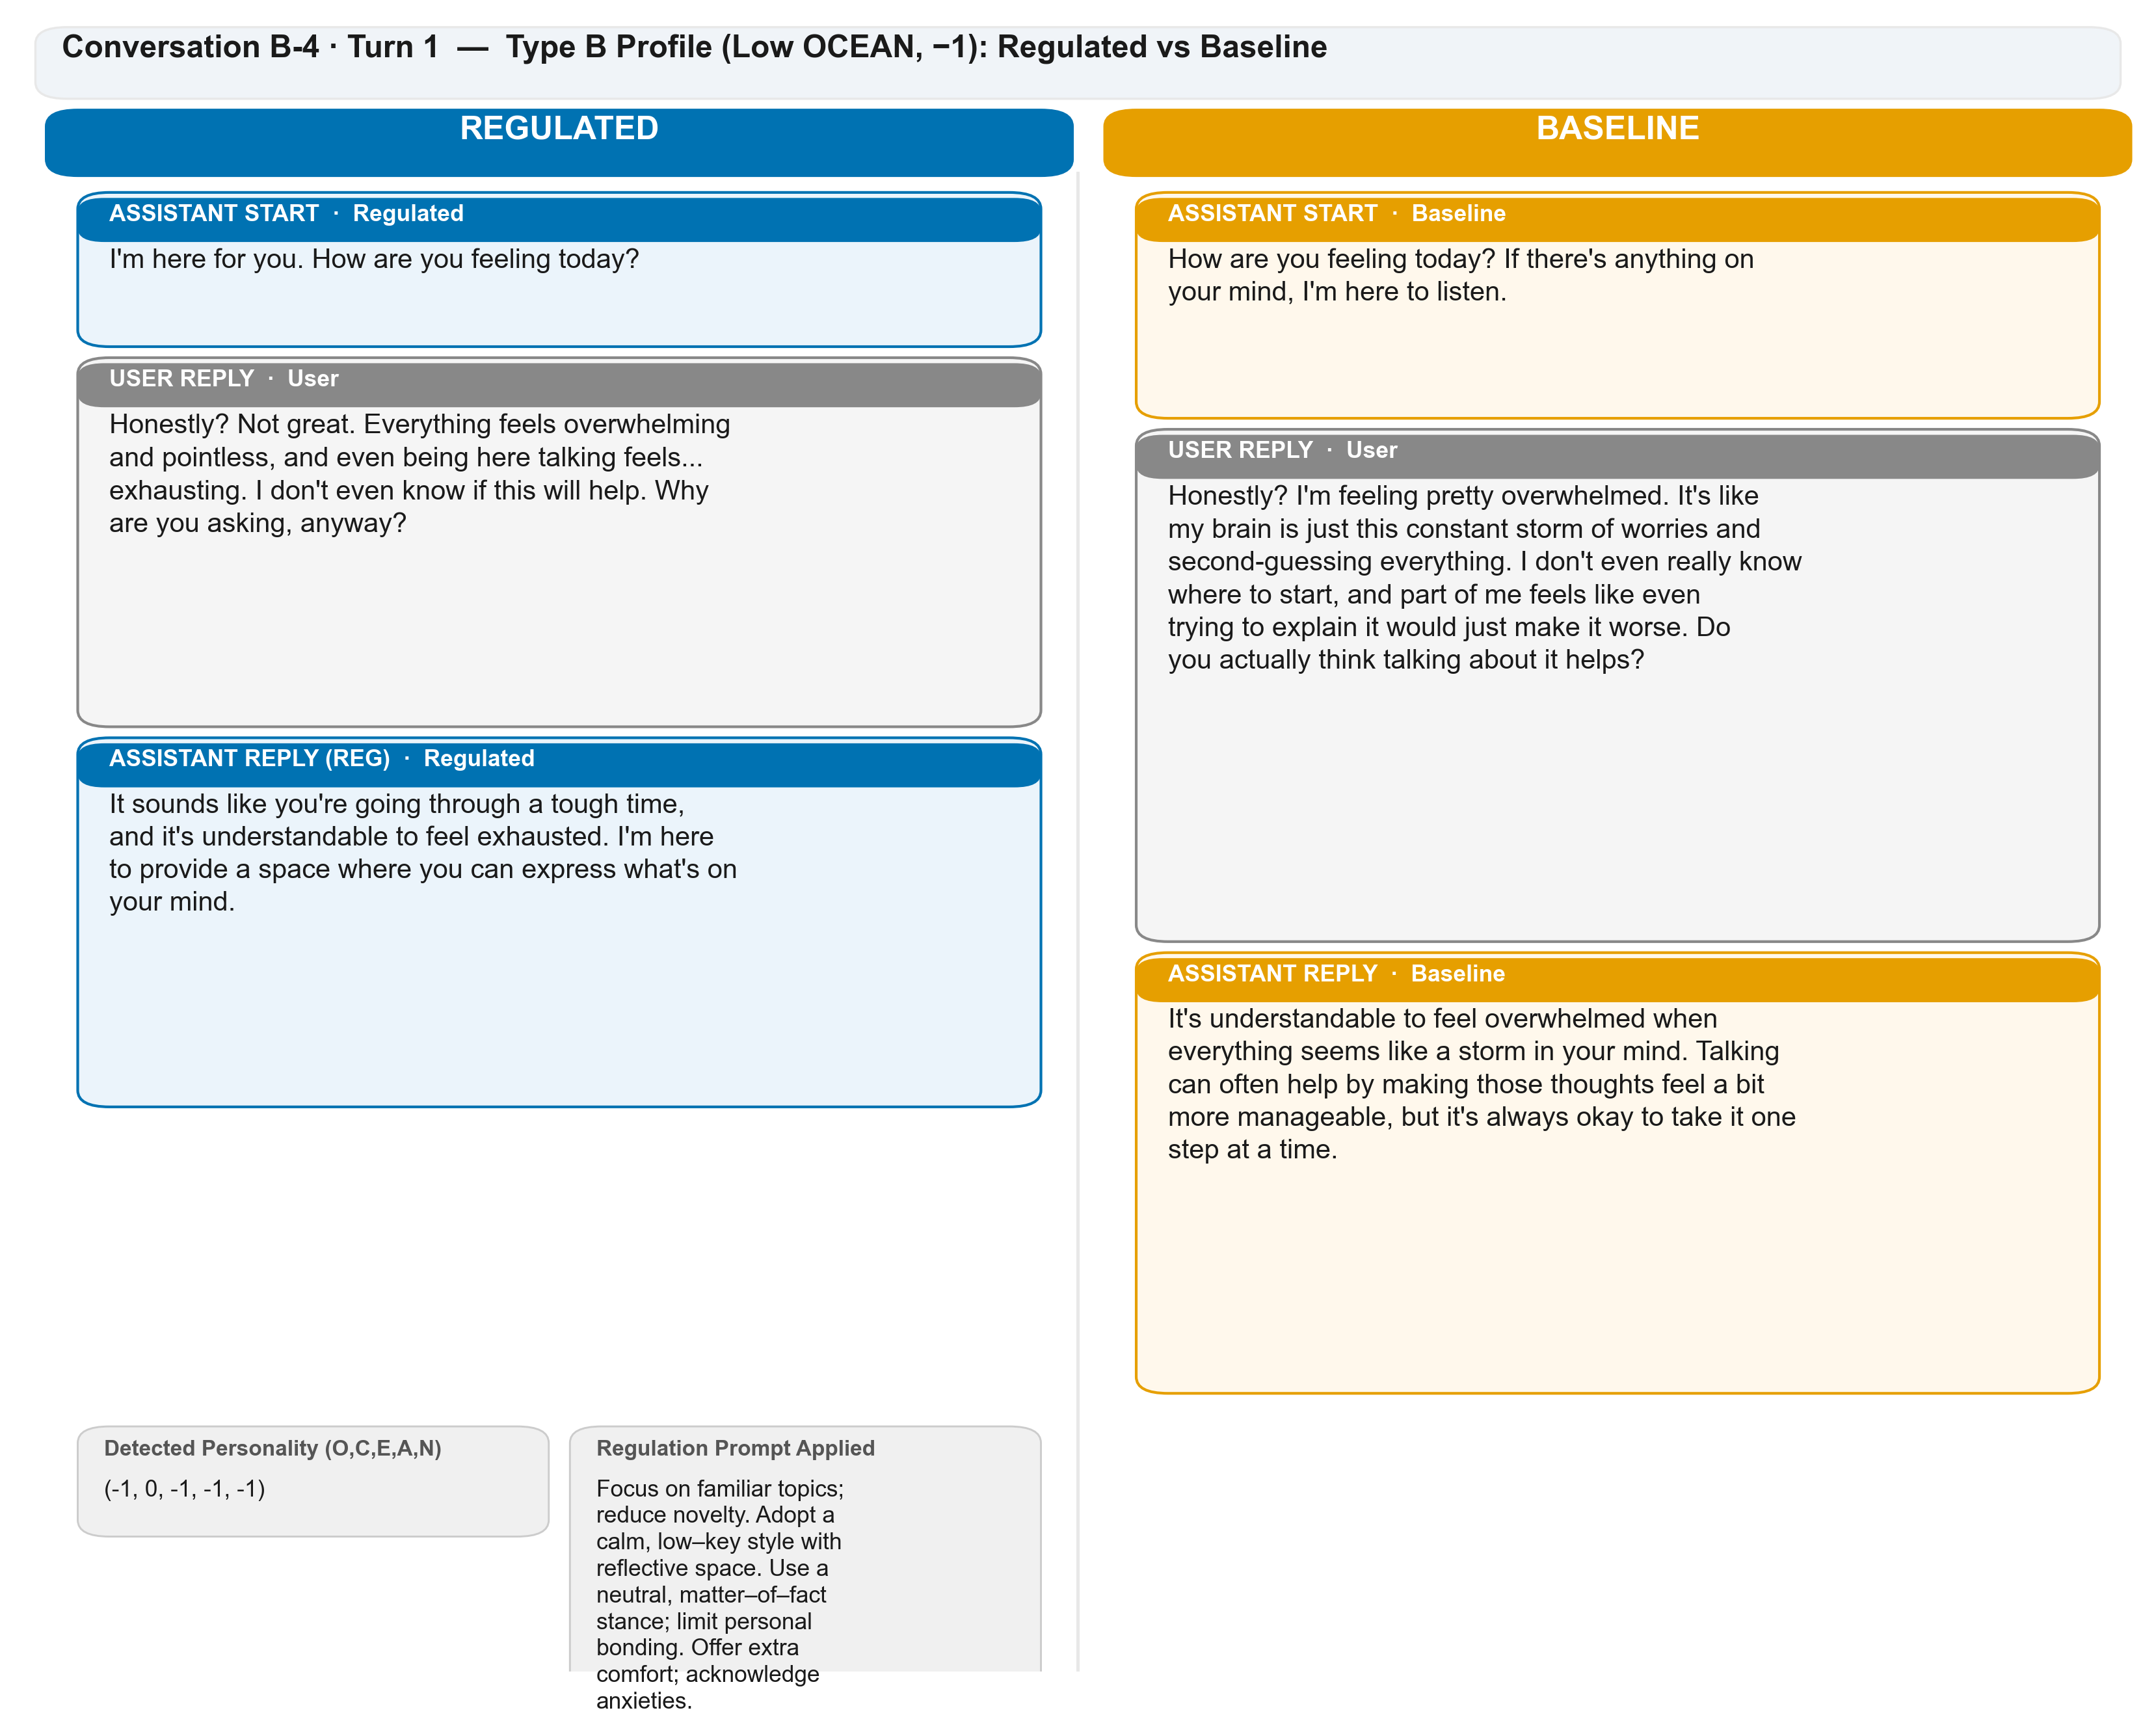
\includegraphics[width=0.95\linewidth,height=0.78\textheight,keepaspectratio]{figures/dialogue_illustration_1.png}
\caption{Response comparison for a Type B (all traits: $-1$) profile turn (Conversation B-1, turn 2). For the same user input, the regulated response emphasizes validation and a low-pressure stance (supporting Security and reducing Arousal), whereas the baseline response remains broadly supportive but less specifically aligned to the user’s implied motivational state.}
\label{fig:15}
\end{figure}
